% !TeX root = ../thesis.tex
\chapter{Exercise Tools}
\label{chp:exercise-tools}
The previous chapter established that the tools currently used for arithmetic research do their job as research instruments but fail as experiences for the children who use them. They lack the motivational, adaptive, and visual qualities that keep children engaged across multiple sessions, and the programming barrier makes it impractical for researchers to add these qualities themselves. The question that follows naturally is: where do these qualities already exist?

The answer is not far away. Across primary schools in Belgium and the Netherlands, children already use digital tools for arithmetic practice on a daily basis. Platforms like Automatus \cite{automatus} and Rekentuin \cite{rekentuin} are designed from the ground up to be engaging, adaptive, and easy for children to use. They look like games, they feel like games, and children are willing to spend time on them without being asked twice. In other words, these tools already solve many of the problems identified in Section \ref{sec:why-this-matters}: they offer the ecological validity, the sustained motivation, and the familiarity that research experiments lack.

This chapter examines exercise tools as a possible solution direction. It begins by defining what makes a good exercise tool, then walks through two prominent examples in the field, and ends by asking the inevitable follow-up question: if exercise tools solve the engagement problem, can they also serve as research tools? The answer, as will become clear, is not quite.

\section{What a good exercise tool needs}
\label{sec:exercise-properties}
Where Section \ref{sec:research-properties} asked what a research tool needs, this section asks the same question for the other side: what makes a good tool for arithmetic practice in the classroom? The properties listed below were developed through discussions with primary school teachers, educational researchers, and the co-supervisor of this thesis. They are not claimed to be exhaustive, but together they capture what practitioners in the field consistently identify as important. Where possible, connections to the educational psychology literature are drawn to ground these observations in theory.

\paragraph{Adaptivity}
Perhaps the single most important property of a good exercise tool is that it adapts to the child using it. Not every child in a classroom is at the same level, and a tool that presents the same exercises to everyone will inevitably bore the strongest students and frustrate the weakest ones. 

This idea has deep theoretical roots: Vygotsky's zone of proximal development (ZPD) is the gap between what a child can do on their own and what they can do with a little help \cite{vygotsky1978mind}. Csikszentmihalyi's flow theory makes a closely related point about engagement more generally, namely that people concentrate best when the difficulty of a task is well-matched to their skill level \cite{csikszentmihalyi1990flow}. In the specific case of arithmetic learning apps for young children, this is more than theory: Bang, Li, and Flynn showed that an adaptive arithmetic app produced significantly larger learning gains and stronger engagement than a non-adaptive control \cite{bang2023mymathacademy}. An exercise tool that does not adapt is, in effect, guaranteeing that most of the children using it will be working below or above their level most of the time.

\paragraph{Engagement}
Adaptivity keeps the difficulty right, but it does not on its own make a child want to open the tool again tomorrow. Engagement is about everything else that makes the experience feel worthwhile: a story that gives context to the exercises, visual rewards for progress, puzzles to unlock, a character to interact with. These are gamification elements, and systematic reviews of gamification in education consistently find that elements such as points, levels, narrative framing, and immediate feedback improve motivation and engagement in mathematics \cite{manzanoleon2021gamification}. For an exercise tool aimed at primary school children, engagement is not optional. A tool that children do not want to use is a tool that does not get used, regardless of how well-designed its exercises are.

\paragraph{Feedback}
Children need to know whether they got the answer right, and ideally they need to know it immediately. Delayed or absent feedback leaves the child uncertain about whether they are learning, and it removes one of the most natural drivers of improvement: the desire to correct a mistake you just made. Meta-analyses of educational feedback confirm that corrective, computer-delivered feedback is among the most effective forms, particularly for new skills \cite{wisniewski2020power}. Interestingly, more is not always better: in a recent study with elementary children, feedback that simply showed the correct answer led to greater persistence and more flexible strategy use than feedback that also added an explicit ``right/wrong'' verification cue \cite{merrick2024feedback}. The key is that feedback is timely, clear, and meaningful.

\paragraph{Personalisation}
Personalisation gives the child the feeling that the tool is theirs. This has two sides. The first is functional: letting children choose which type of exercise to practise, whether they want to see a timer, or what difficulty level they prefer. This kind of choice can give children a sense of ownership: a child who decides to practise multiplication because they know it is their weakest area is doing something more valuable than just answering another question. The second side is personal identity: an avatar, a nickname, a progress tracker that shows their journey, a customised home screen. These elements may seem cosmetic, but they transform a generic program into something that feels like it belongs to the child, which in turn makes the child more likely to come back to it \cite{cordova1996intrinsic}.

\paragraph{Accessibility}
An exercise tool is only useful if children can actually reach it. In practice this means the tool should run in a web browser, work on the devices that schools actually have (laptops, tablets, Chromebooks), and not require any software installation. It also means the tool should be available outside the classroom, so that children can practise at home if they want to. 

\paragraph{User friendliness}
Finally, the tool has to be usable by its target audience, which in this case is children between roughly seven and eleven years old. This means large buttons, clear icons, simple navigation, and a visual language that children understand without needing instructions. Every unnecessary interface element adds extraneous cognitive load, the kind of mental effort that does not contribute to learning, and so takes working memory away from the actual exercise \cite{mayer2003nine}. 

\section{Existing exercise tools: Automatus and Rekentuin}
\label{sec:exercise-tools}

\subsection{Automatus}
Automatus \cite{automatus} is a web-based arithmetic practice platform used in primary schools across Flanders and the Netherlands. It was designed with a clear purpose: to help children automate their arithmetic skills through repeated, structured practice. Teachers assemble customised ``lands'' consisting out of tiles, where each tile corresponds to a specific type of problem (for example, additions up to 20, or the multiplication table of 7). Children then work their way through these tiles, with the map giving each session a visible sense of direction and progression. Figure~\ref{fig:automatus_ui} shows the tile screen children encounter while practising.

\begin{figure}
\centering
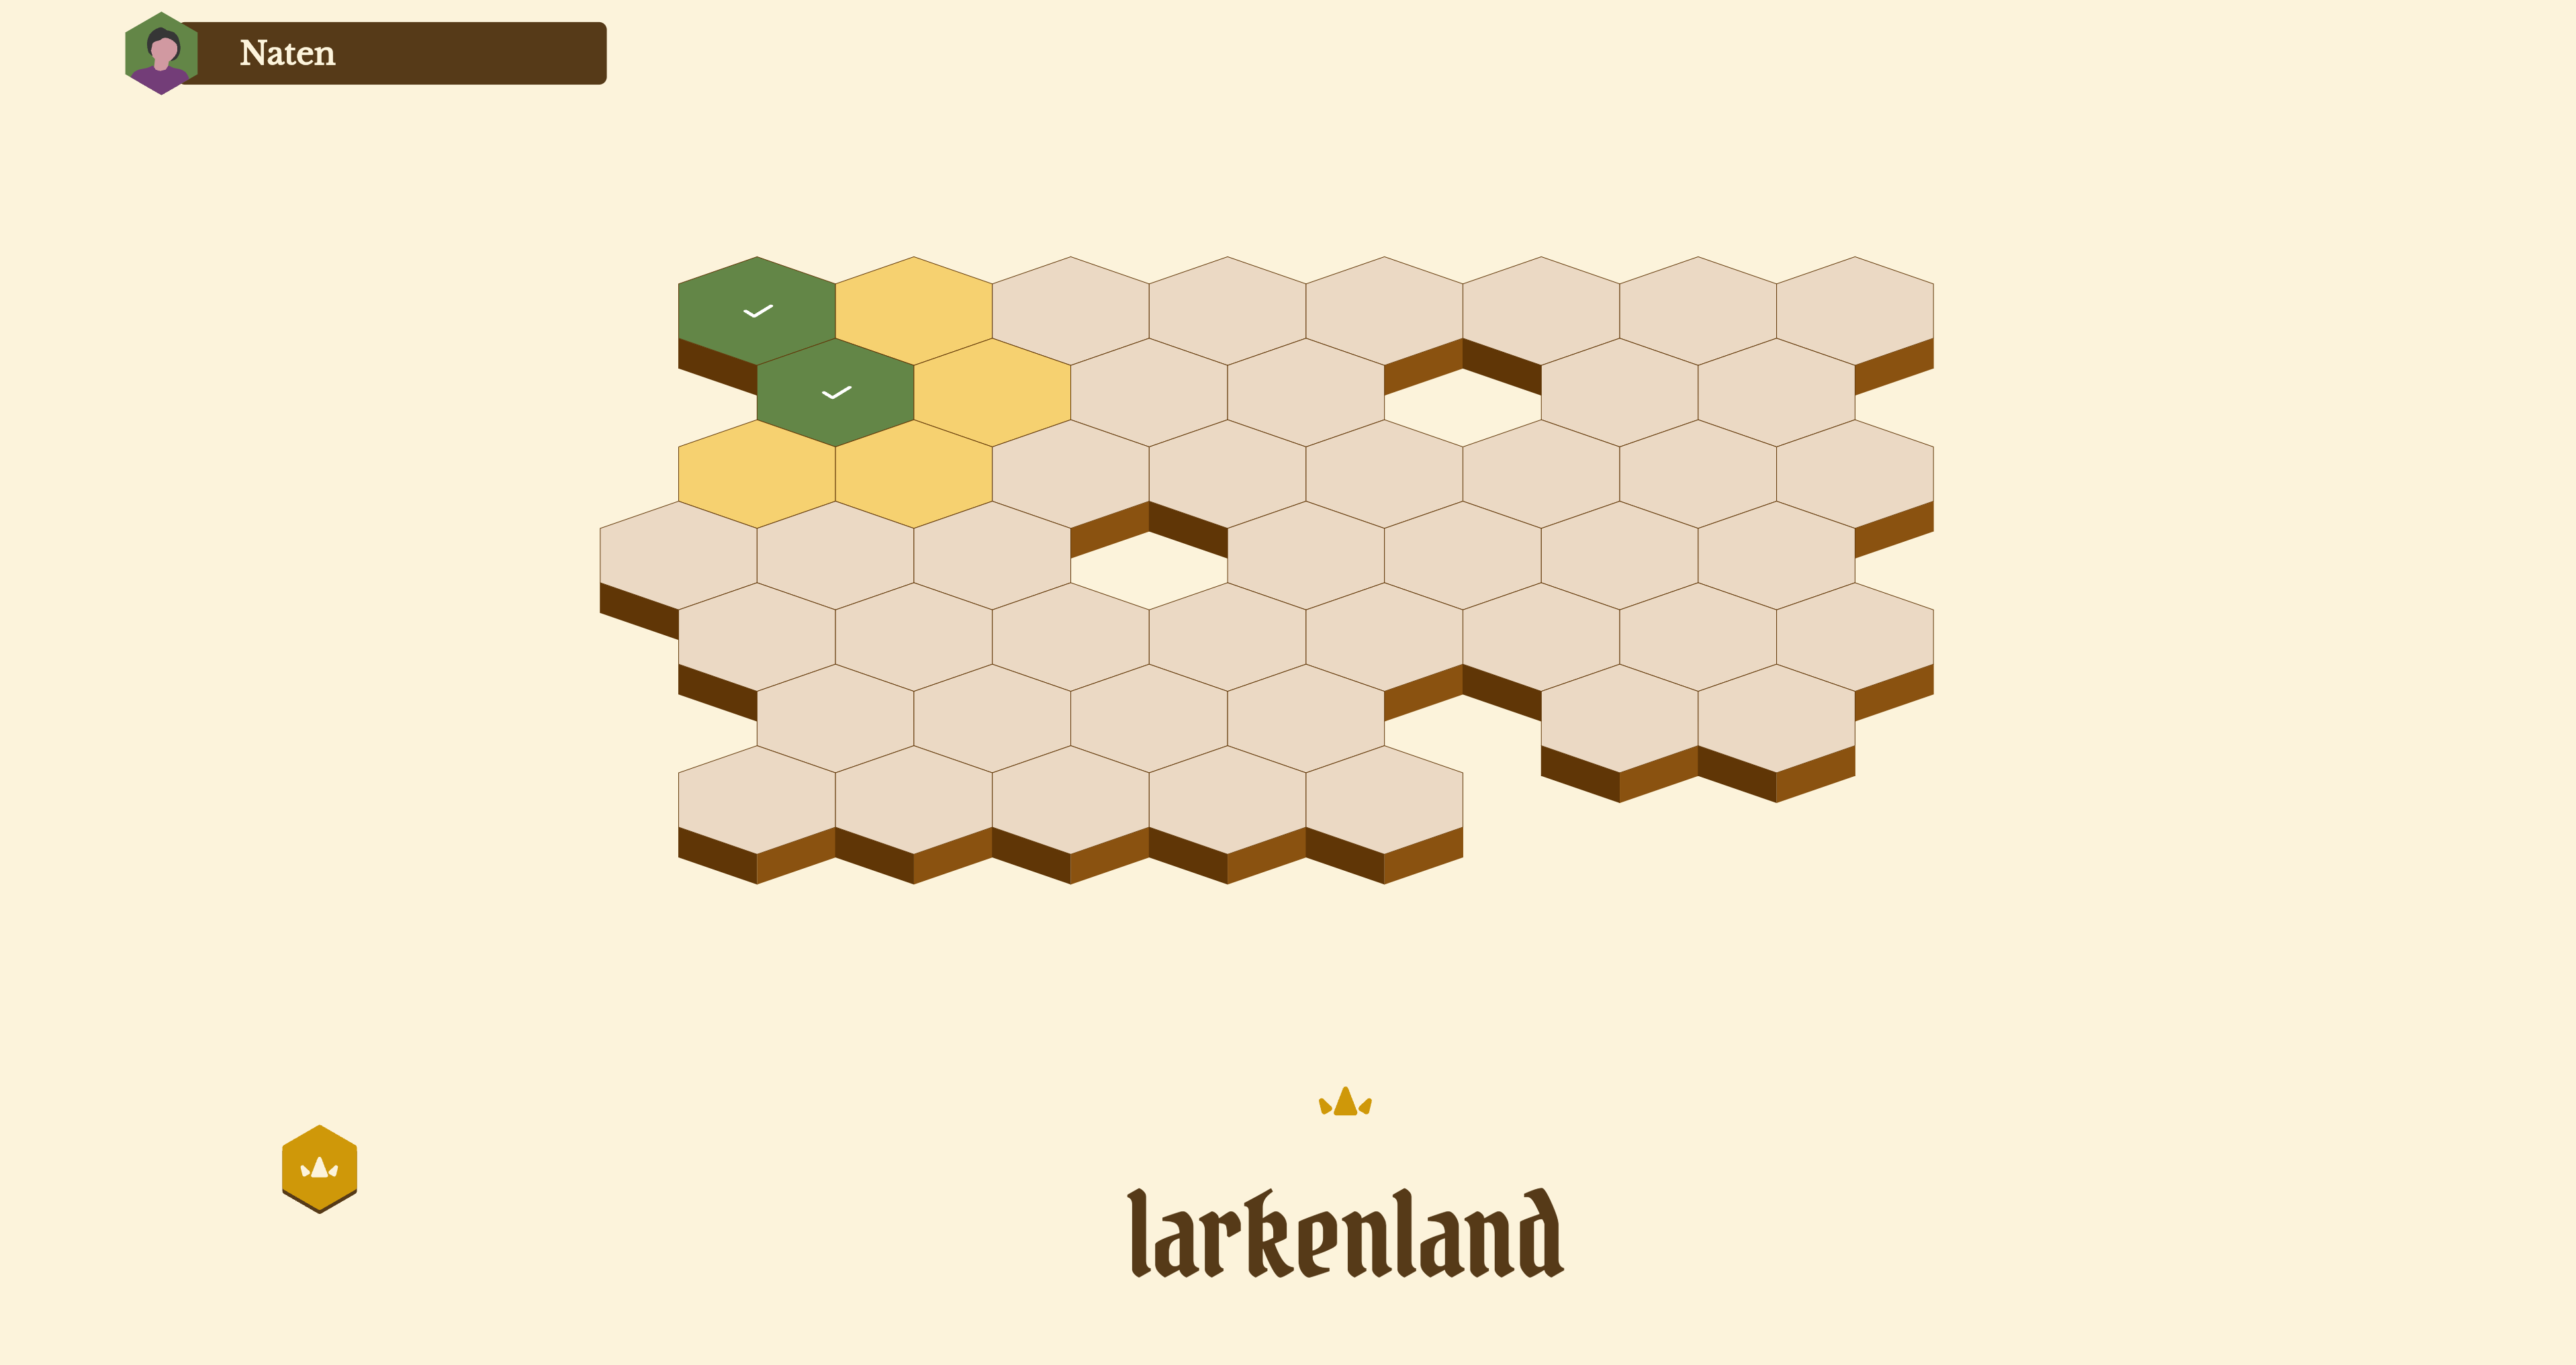
\includegraphics[width=0.85\textwidth]{figures/automatus_ui.png}
\caption{Screenshot of the Automatus interface from the pupil's perspective, showing the tile-based landscape through which learners navigate exercises.}
\label{fig:automatus_ui}
\end{figure}

On the six exercise-tool properties from Section \ref{sec:exercise-properties}, Automatus scores well on five of them. \textbf{Adaptivity} is handled in a specific way: rather than adjusting the difficulty of the exercises, Automatus adapts the goal time the child has to answer them. This is what the platform calls \textit{adaptive automatisation} as opposed to \textit{adaptive practice}, and it positions itself as one of the first platforms built around this distinction\footnote{\url{https://automatus.be/scholen/faq/wat-is-adaptief-automatiseren/}}. \textbf{Engagement} is supported by the map-and-tile structure, which gives children a visible sense of progress, and by response-time tracking that lets them compare their current attempt against their personal best, adding a layer of self-competition. \textbf{Feedback} is well-handled: when a child answers incorrectly, the exercise progress pauses and the platform shows a short explanation of the correct approach. \textbf{Accessibility} is excellent: Automatus runs in any browser and is also available as a tablet application, so it works on the devices schools and families actually have. \textbf{User friendliness} is equally strong: the interface is clean and intuitive enough that children can navigate it without adult help.

The one property where Automatus does not fully deliver is \textbf{personalisation}. The functional side is partially present: children can in some cases choose which exercises they want to work on, and the performance tracking gives a sense of individual progress. But the identity side is missing: there is no avatar, no personal profile beyond a name, no visual element that makes the tool feel like it belongs to the child rather than to the classroom. This is a minor gap in an otherwise very well-designed tool.

\subsection{Rekentuin}
Rekentuin (Math Garden) is a web-based arithmetic learning environment developed at the University of Amsterdam by Straatemeier, Klinkenberg, and van der Maas \cite{straatemeier2014mathgarden}. From the start it was built with a dual purpose: serving children as a practice platform and serving researchers as a scientific instrument for studying arithmetic development \cite{straatemeier2014mathgarden}. It has grown into one of the most widely used arithmetic tools in the Netherlands, with more than 400,000 primary school children practising on it \cite{brinkhuis2018learning}, and is now maintained and distributed as part of the Prowise Learn \cite{prowiselearn}.

The platform organises its content around a world map with multiple thematic islands, each representing a different mathematical domain. Children navigate between islands and work through exercises that range from basic addition to fractions and percentages. Figure~\ref{fig:rekentuin_ui} shows the main interface.

\begin{figure}
\centering
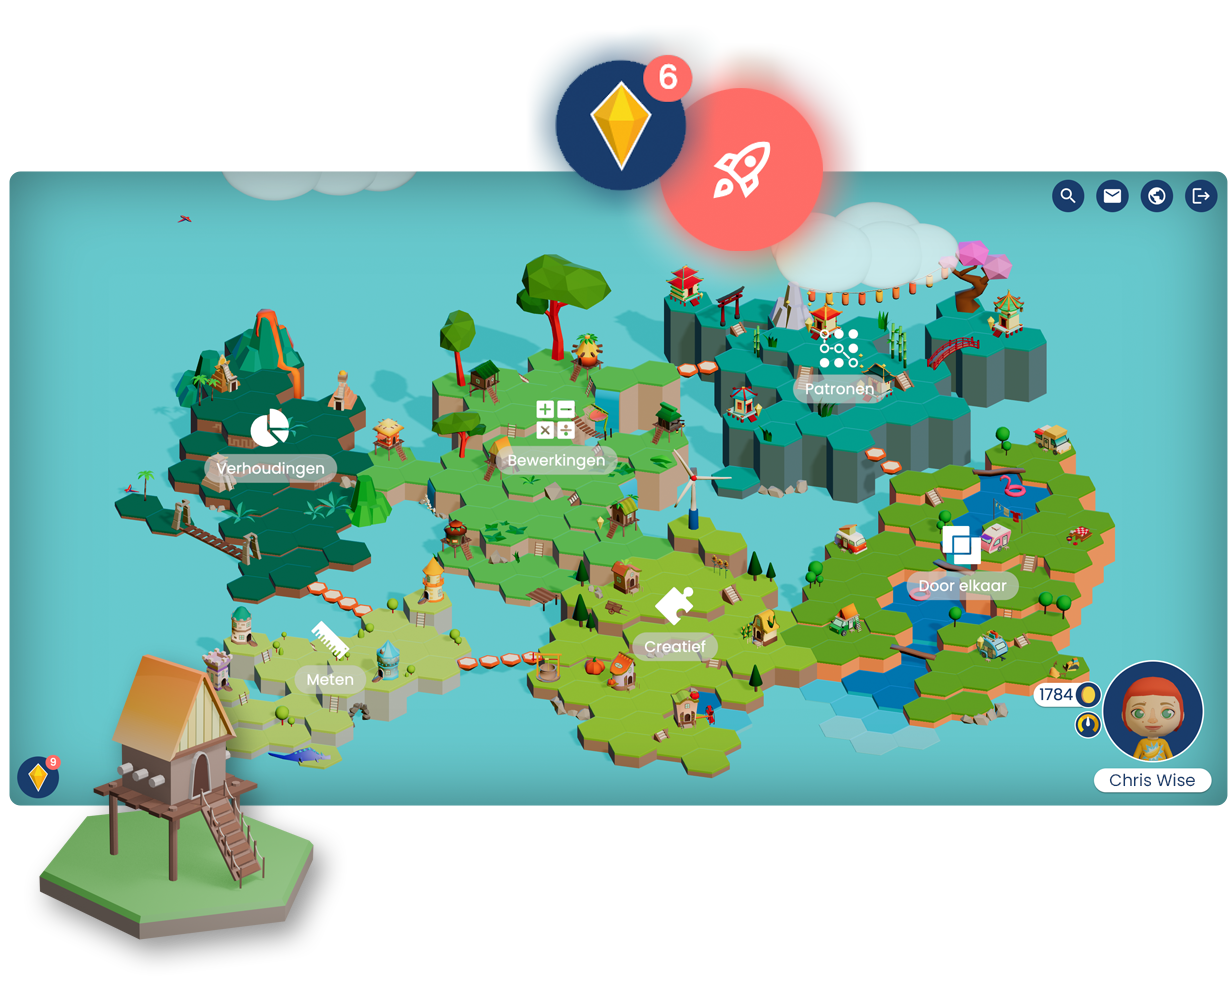
\includegraphics[width=0.85\textwidth]{figures/Rekentuin.png}
\caption{Screenshot of the Rekentuin interface from the pupil's perspective, showing the different continents from which learners can select different exercises.}
\label{fig:rekentuin_ui}
\end{figure}

On the six properties, Rekentuin delivers strongly across the board. \textbf{Adaptivity} is the cornerstone of the platform's design. Rekentuin's adaptive engine combines the Elo rating system with an item response model, continuously estimating how able each child is and how hard each item is, and then choosing items so that the child answers correctly with a probability of roughly 75\% \cite{klinkenberg2011computer}. Children can also choose between three difficulty levels within each game, adding a layer of self-regulation on top of the algorithm. \textbf{Engagement} is sustained through the island-based world, a variety of games across different mathematical topics, and a coin system: faster and more accurate answers earn more coins. The platform also highlights recommended games and ``super games'' based on the child's performance, gently steering practice toward areas that need attention. \textbf{Feedback} is immediate. Children see whether their answer was correct after each problem, and the coin reward provides a secondary signal of how well they performed relative to the time limit. \textbf{Personalisation} is where Rekentuin distinguishes itself most clearly from Automatus. The coins children earn are tied to an avatar that they can dress, decorate, and customise, giving every child a visible, personal identity within the platform. Combined with the personalised game recommendations and the self-selected difficulty levels, the experience feels suited to each individual. \textbf{Accessibility} is strong: Rekentuin runs in any web browser, including on mobile devices, and data from Klinkenberg et al. show that children completed roughly a third of their exercises outside school hours \cite{klinkenberg2011computer}, indicating that the platform is genuinely used at home as well as in the classroom. \textbf{User friendliness} is well-designed for the target age group, with large interactive elements, colourful visuals, and a navigation structure built around the world and islands that children understand intuitively.

At this point, a similar comparison to the one drawn for OpenSesame and PsychoPy in Section \ref{sec:research-tools} is useful. Figure~\ref{fig:exercise-tool-grid} evaluates both Automatus and Rekentuin against the six exercise-tool properties. Automatus falls just short on personalisation, while Rekentuin delivers on all six. These tools do exactly what they were designed to do. The question that follows is whether they can also serve the needs of researchers. That is the subject of the next section.

\begin{figure}
\centering
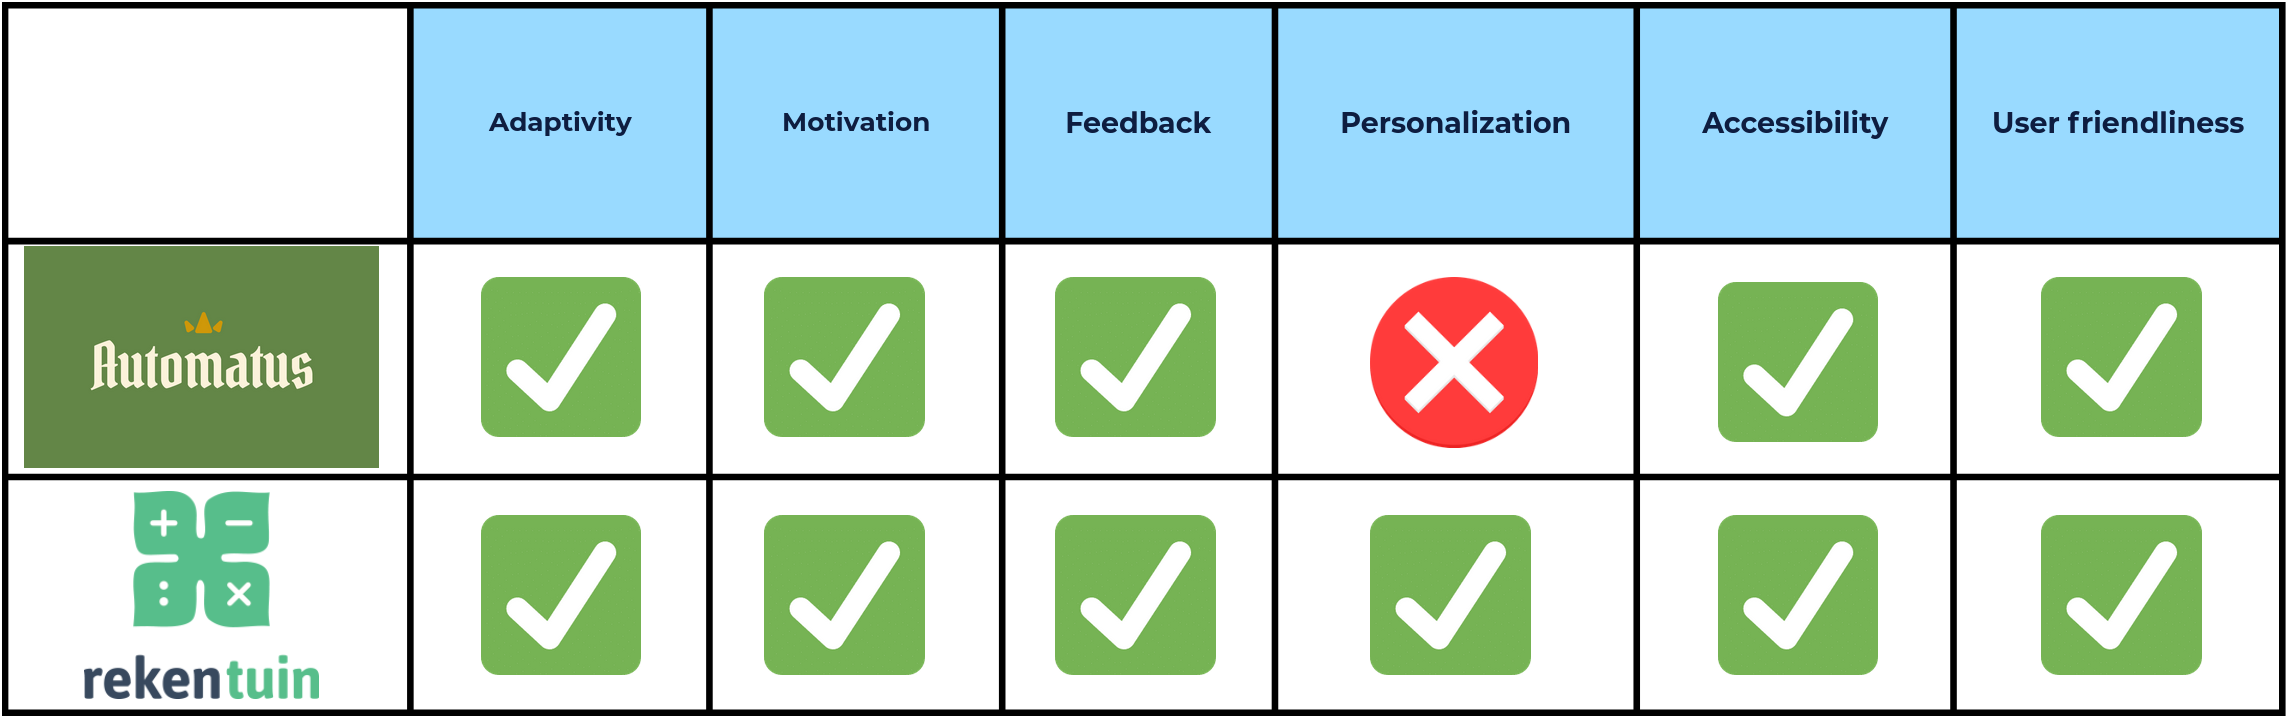
\includegraphics[width=0.85\textwidth]{figures/grid_exercise.png}
\caption{Automatus and Rekentuin evaluated against the six exercise-tool properties from Section \ref{sec:exercise-properties}. Both perform well across the board; Automatus falls slightly short on personalisation.}
\label{fig:exercise-tool-grid}
\end{figure}

\section{Why exercise tools alone are not the answer}
\label{sec:not-the-answer}
The previous section showed that Automatus and Rekentuin are excellent exercise tools. They are adaptive, engaging, well-designed, and genuinely enjoyed by children. A natural question follows: if these tools already solve the engagement and motivation problems that plague research tools, could they not simply be used for research as well?

To answer this, the same six research-tool properties from Section \ref{sec:research-properties} can be applied to both platforms. The result, summarised alongside the exercise-tool evaluation in Figure~\ref{fig:combined-grid}, shows a clear pattern. On three of the six research properties, both tools perform well. On the other three, they fall short in ways that matter.

The three properties that hold up are straightforward. \textbf{Reproducibility} is well-supported: once a teacher has configured a set of exercises for a class, that configuration is saved and can be reused next semester without effort. \textbf{Reliability} is equally strong. Both Automatus and Rekentuin are mature, commercially maintained products used daily by hundreds of thousands of children. They are stable, they do not crash mid-session, and they behave consistently across devices. \textbf{Ease of setup} is, unsurprisingly, a strength rather than a weakness. Both tools were built for teachers, not programmers. Setting up a class, assigning exercises, and managing student progress is done entirely through a graphical dashboard with no code involved.

The problems emerge in the remaining three properties. \textbf{Data tracking} is the first issue. Both platforms collect data on student performance, and teachers can see summaries of accuracy and progress over time. But the level of detail is not what a researcher needs. Arithmetic research requires the exact response time for every individual trial, the precise answer the child gave (not just whether it was correct), and ideally the timestamp of every screen transition. These fine-grained data points are what allow researchers to distinguish, for example, between a child who retrieved a fact from memory in under two seconds and one who calculated the answer in five. Exercise tools log enough to inform a teacher; they do not always log enough to inform a study.

\textbf{Experimental control} is the second and arguably most fundamental problem. As discussed in Section \ref{sec:research-properties}, controlled experiments depend on the researcher being able to dictate what each participant sees and under what conditions. Exercise tools are designed around a partly opposite principle: they are built to give children autonomy, with the system adapting on its own and the teacher setting broad goals rather than trial-by-trial sequences. Some features can be configured by the teacher, and it is not impossible to get two children to see the same set of exercises. But for the kind of fine-grained control a research design typically needs (disabling specific features for a single group, forcing a fixed item sequence, switching off adaptivity while keeping everything else the same) the platforms simply were not designed with this in mind, and the level of control an OpenSesame-style tool offers is out of reach.

\textbf{Flexibility} is the third gap, and it is closely tied to the previous one. As also discussed in Section \ref{sec:research-properties}, flexibility in a research context is the ability to set up a wide range of experimental designs without rebuilding the tool. The configuration options exercise tools expose are designed for pedagogical goals, not experimental ones. A researcher who wants to swap the adaptive algorithm for a different one, introduce a new kind of task, or restructure the session into multi-block sequences with custom rules between blocks has no way to express any of that within the platforms. The kind of flexibility a programming language offers is absent, and the graphical interface itself was never built to support the structured designs that some research studies require.

Figure~\ref{fig:combined-grid} brings both evaluations together. The research-tool properties are on the left, the exercise-tool properties on the right. Automatus and Rekentuin fill the right side almost entirely with green. The left side tells a different story: reproducibility, reliability, and ease of setup are covered, but data tracking, experimental control, and flexibility are not. Exercise tools, on their own, are not the answer. But the qualities they bring to the table are exactly the qualities that Chapter \ref{chp:background} identified as missing from research tools. The next section brings all four tools and all twelve properties together to make this gap fully visible.

\begin{figure}
\centering
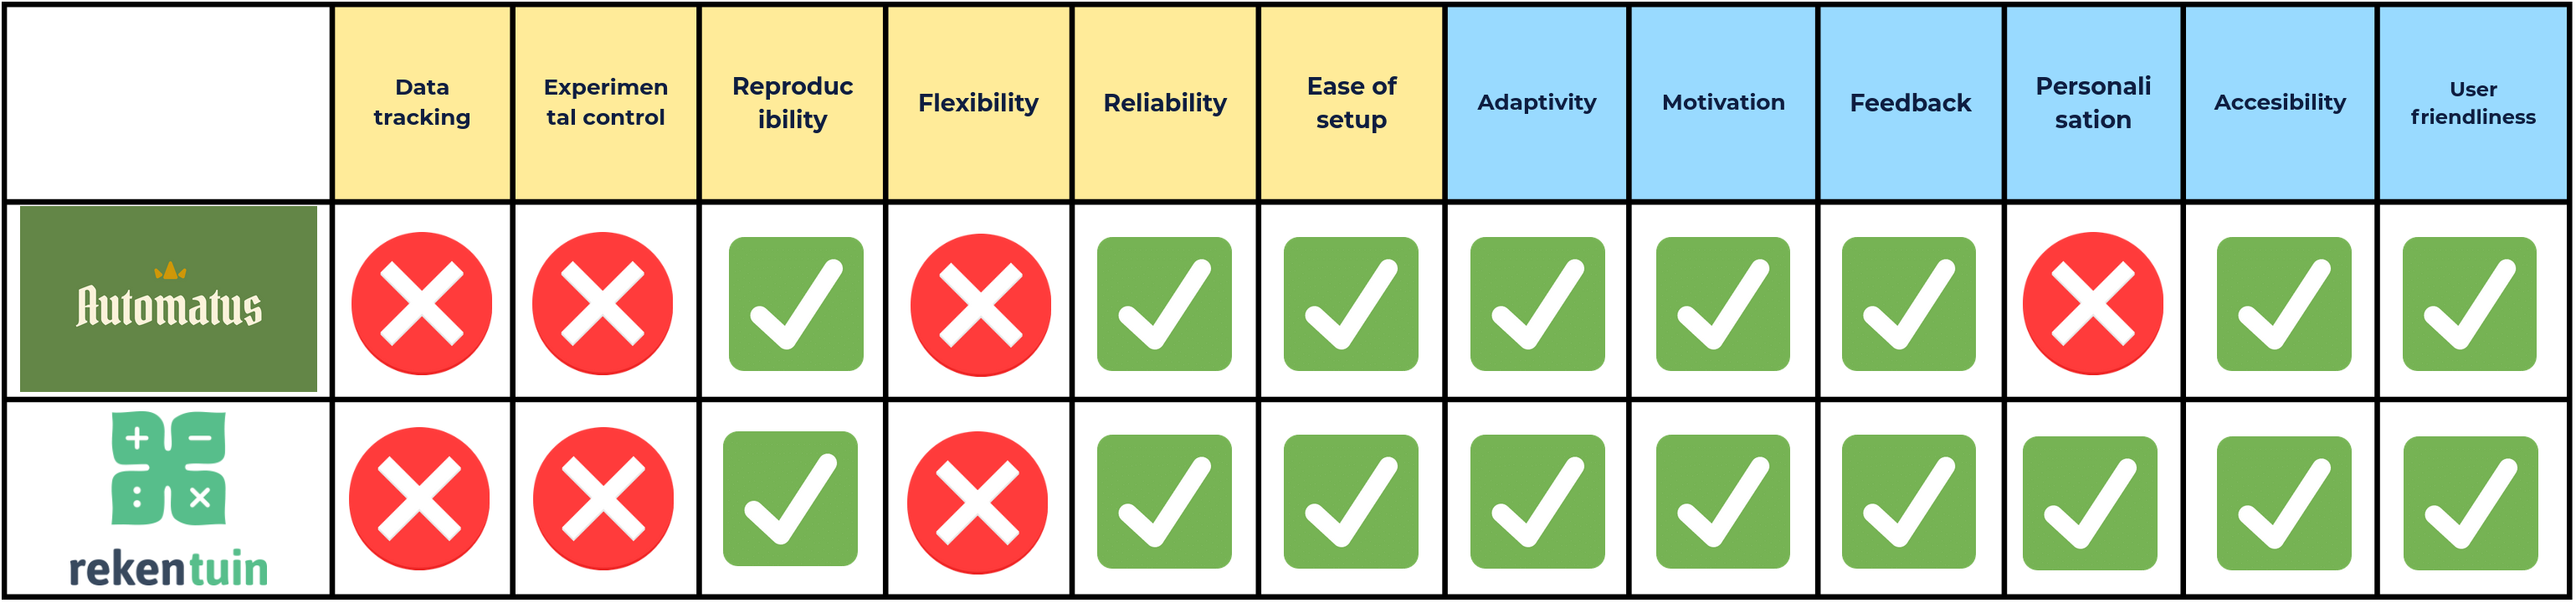
\includegraphics[width=0.85\textwidth]{figures/grid_exercise_research.png}
\caption{Combined comparison of Automatus and Rekentuin against both the exercise-tool properties (Section \ref{sec:exercise-properties}) and the research-tool properties (Section \ref{sec:research-properties}). Both tools excel on the exercise side but fall short on data tracking, experimental control, and flexibility.}
\label{fig:combined-grid}
\end{figure}


\section{The gap: no existing tool covers both sides}
The previous sections built up the comparison piece by piece. Section \ref{sec:research-tools} evaluated OpenSesame and PsychoPy on the research-tool properties, Section \ref{sec:exercise-tools} evaluated Automatus and Rekentuin on the exercise-tool properties, and Section \ref{sec:not-the-answer} tested whether exercise tools could also serve as research tools and found that they could not. The one combination left to make explicit is the reverse: how do the research tools score on the exercise-tool properties?

Section \ref{sec:shared-limitations} answered this question. OpenSesame and PsychoPy were not built to be exercise tools, and they offer none of the six properties from Section \ref{sec:exercise-properties} out of the box. There is no built-in adaptivity, no gamification, no avatar system, no child-friendly login. All of these could in theory be added, but only by writing them from scratch in Python, which brings the researcher straight back to the same programming wall that already made ease of setup the weakest point on the research side.

Figure~\ref{fig:full-grid} brings everything together. All four tools are evaluated against all twelve properties: the six research-tool properties on the left, the six exercise-tool properties on the right. The pattern is now fully visible. Automatus and Rekentuin fill the exercise columns with green but leave gaps in the research columns. OpenSesame and PsychoPy do the reverse. Each tool excels at what it was designed for. None covers both sides.

\begin{figure}
\centering
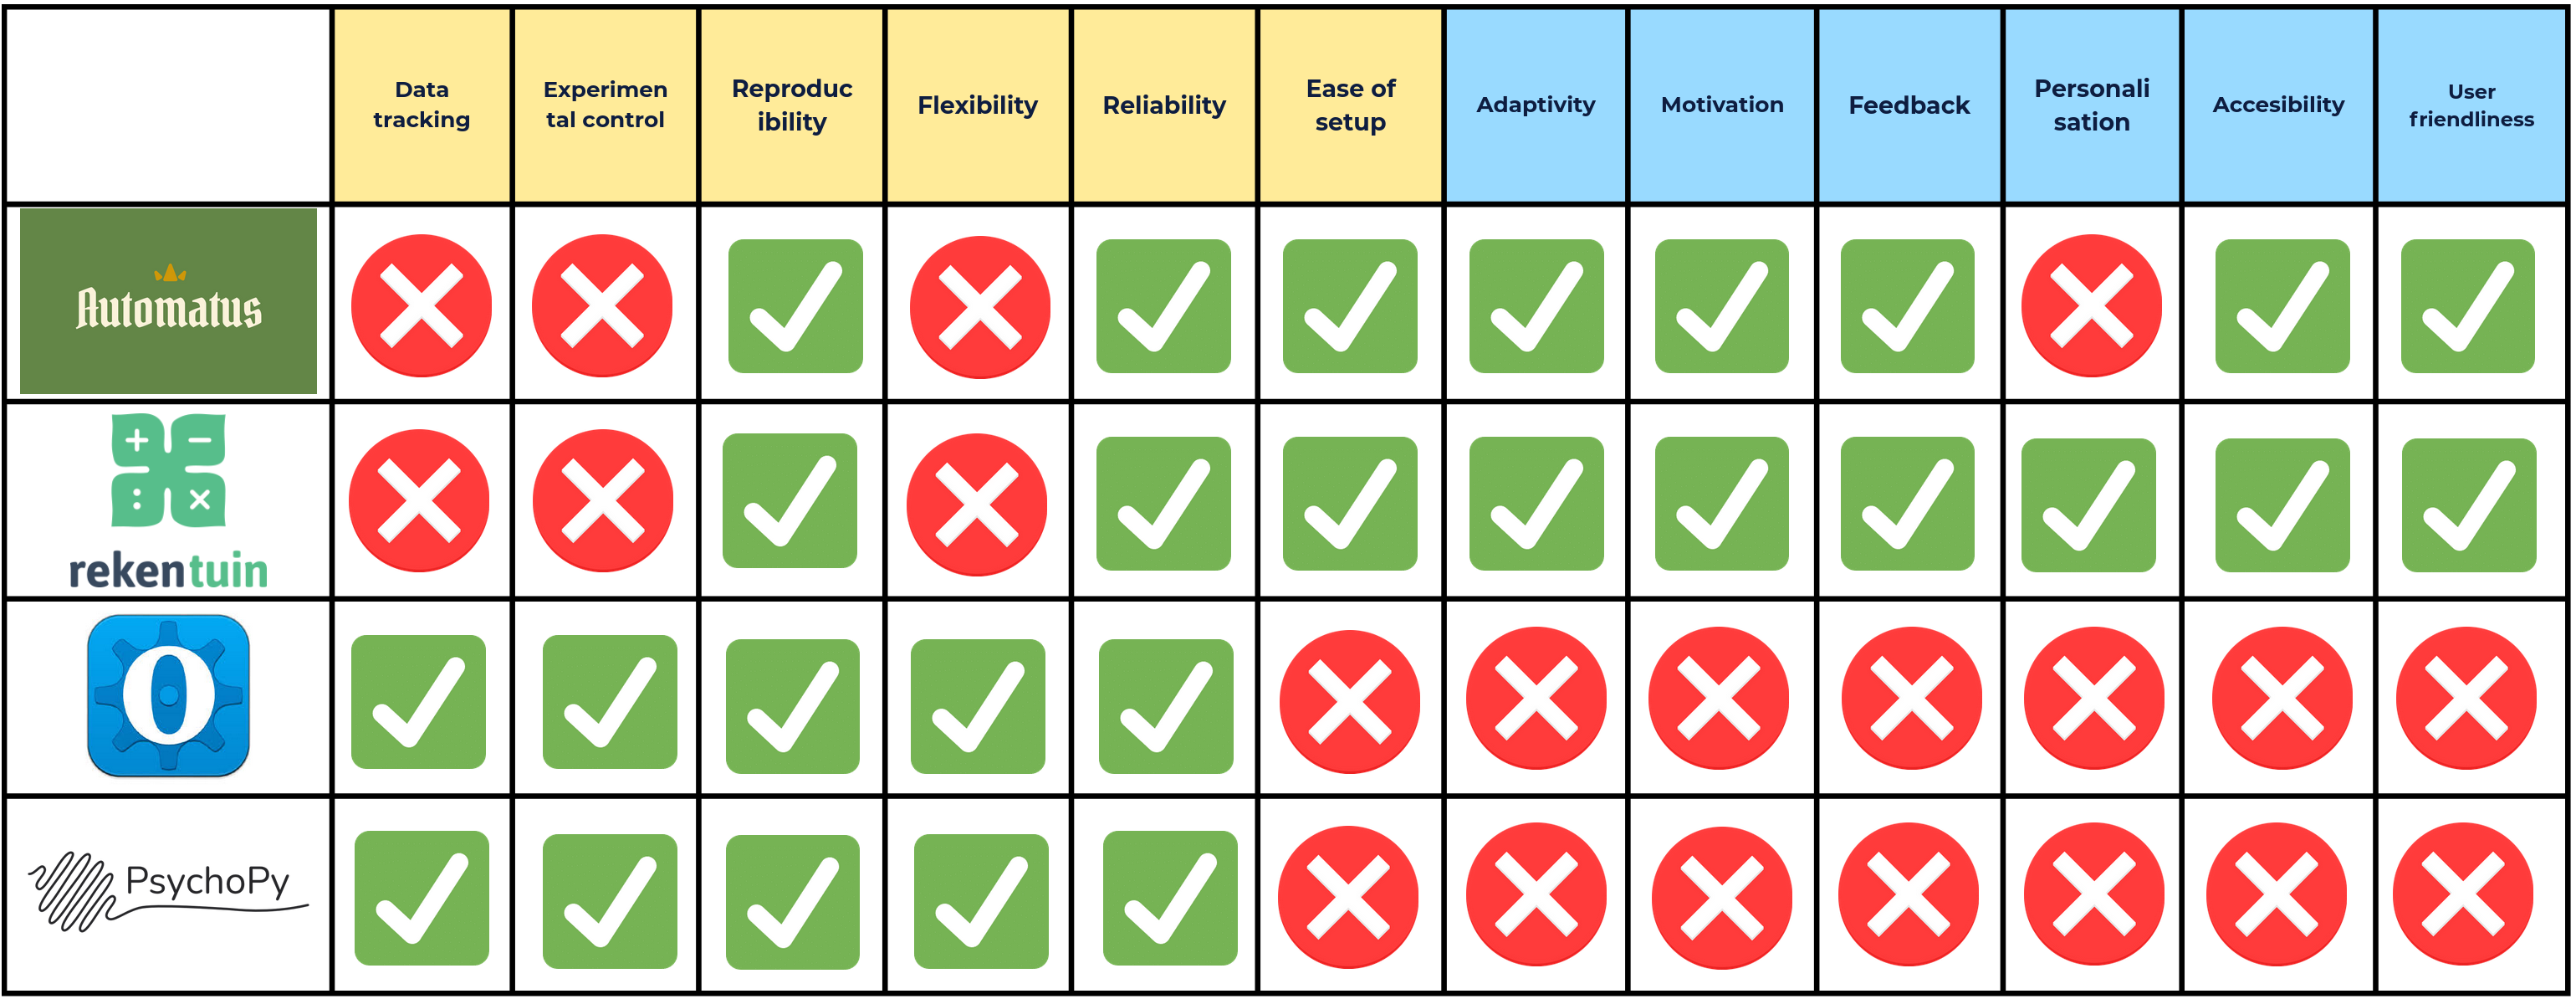
\includegraphics[width=0.85\textwidth]{figures/grid.png}
\caption{Full comparison of all four tools against the twelve properties defined in Sections \ref{sec:research-properties} and \ref{sec:exercise-properties}. Exercise tools (top) score well on exercise properties but lack key research properties. Research tools (bottom) score well on research properties but offer none of the exercise-tool qualities.}
\label{fig:full-grid}
\end{figure}

This is not a criticism of any of these tools individually. Each was built for a specific purpose and serves that purpose well. But for a researcher who wants to run a controlled experiment in a classroom, with children who stay motivated across multiple sessions, using a tool that feels familiar rather than foreign, there is currently no option that works. That gap is formalised in the next chapter.